\documentclass{standalone}

\usepackage{tikz}
\usepackage[outline]{contour}

\begin{document}
  %noformat{
  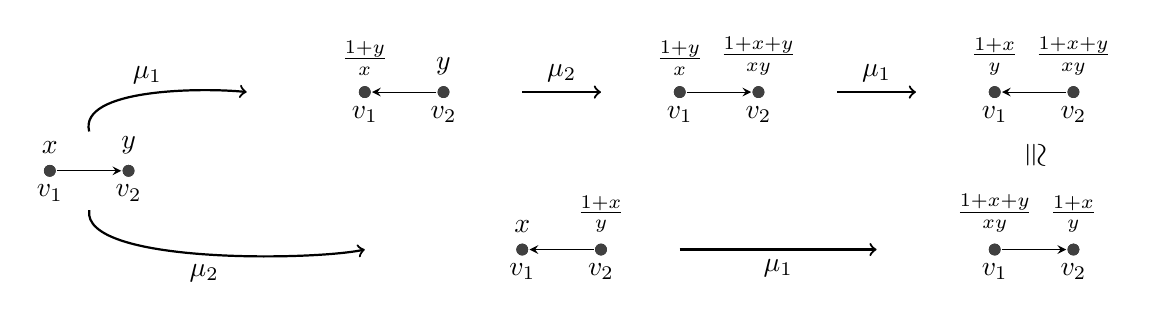
\begin{tikzpicture}
    \contourlength{1.2pt}
    \tikzstyle{v1} = [circle, outer xsep=0.5pt, fill, inner sep=1.5pt]
    \tikzstyle{v2} = [circle, outer xsep=0.5pt, fill, inner sep=3.0pt]
    \tikzstyle{v3} = [circle, outer xsep=0.5pt, fill, inner sep=4.5pt]
    \tikzstyle{unf} = [color=darkgray]
    \tikzstyle{frz} = [color=blue!60!darkgray!70]
    \tikzstyle{e} = [->, >={stealth}, preaction={draw=white, -, ultra thick}]
    \tikzstyle{h} = [dashed, color=gray, ->, >={stealth}]
    \tikzstyle{r} = [->, color=red!70!darkgray!70, >={stealth}]

    % \tikzset{font=\tiny}

    \begin{scope}[shift={( 0.0, 0.0)}]
      \coordinate[v1] (v1) at (0,0);
      \coordinate[v1] (v2) at (1,0);
      \draw[e] (v1) -- (v2);
      \node[v1,label={[label distance=0pt]90:{$x$}},label={[label distance=-1pt]270:{\contour{white}{$v_{1}$}}}, unf] (n_v1) at (v1) {};
      \node[v1,label={[label distance=0pt]90:{$y$}},label={[label distance=-1pt]270:{\contour{white}{$v_{2}$}}}, unf] (n_v2) at (v2) {};
    \end{scope}

    % left
    \begin{scope}[shift={( 4.0, 1.0)}]
      \coordinate[v1] (v1) at (0,0);
      \coordinate[v1] (v2) at (1,0);
      \draw[e] (v2) -- (v1);
      \node[v1,label={[label distance=0pt]90:{$\frac{1+y}{x}$}},label={[label distance=-1pt]270:{\contour{white}{$v_{1}$}}}, unf] (n_v1) at (v1) {};
      \node[v1,label={[label distance=0pt]90:{$y$}},label={[label distance=-1pt]270:{\contour{white}{$v_{2}$}}}, unf] (n_v2) at (v2) {};
    \end{scope}

    \begin{scope}[shift={( 8.0, 1.0)}]
      \coordinate[v1] (v1) at (0,0);
      \coordinate[v1] (v2) at (1,0);
      \draw[e] (v1) -- (v2);
      \node[v1,label={[label distance=0pt]90:{$\frac{1+y}{x}$}},label={[label distance=-1pt]270:{\contour{white}{$v_{1}$}}}, unf] (n_v1) at (v1) {};
      \node[v1,label={[label distance=0pt]90:{$\frac{1+x+y}{xy}$}},label={[label distance=-1pt]270:{\contour{white}{$v_{2}$}}}, unf] (n_v2) at (v2) {};
    \end{scope}

    \begin{scope}[shift={(12.0, 1.0)}]
      \coordinate[v1] (v1) at (0,0);
      \coordinate[v1] (v2) at (1,0);
      \draw[e] (v2) -- (v1);
      \node[v1,label={[label distance=0pt]90:{$\frac{1+x}{y}$}},label={[label distance=-1pt]270:{\contour{white}{$v_{1}$}}}, unf] (n_v1) at (v1) {};
      \node[v1,label={[label distance=0pt]90:{$\frac{1+x+y}{xy}$}},label={[label distance=-1pt]270:{\contour{white}{$v_{2}$}}}, unf] (n_v2) at (v2) {};
    \end{scope}

    % right
    \begin{scope}[shift={( 6.0,-1.0)}]
      \coordinate[v1] (v1) at (0,0);
      \coordinate[v1] (v2) at (1,0);
      \draw[e] (v2) -- (v1);
      \node[v1,label={[label distance=0pt]90:{$x$}},label={[label distance=-1pt]270:{\contour{white}{$v_{1}$}}}, unf] (n_v1) at (v1) {};
      \node[v1,label={[label distance=0pt]90:{$\frac{1+x}{y}$}},label={[label distance=-1pt]270:{\contour{white}{$v_{2}$}}}, unf] (n_v2) at (v2) {};
    \end{scope}

    \begin{scope}[shift={(12.0,-1.0)}]
      \coordinate[v1] (v1) at (0,0);
      \coordinate[v1] (v2) at (1,0);
      \draw[e] (v1) -- (v2);
      \node[v1,label={[label distance=0pt]90:{$\frac{1+x+y}{xy}$}},label={[label distance=-1pt]270:{\contour{white}{$v_{1}$}}}, unf] (n_v1) at (v1) {};
      \node[v1,label={[label distance=0pt]90:{$\frac{1+x}{y}$}},label={[label distance=-1pt]270:{\contour{white}{$v_{2}$}}}, unf] (n_v2) at (v2) {};
    \end{scope}

    \draw[->, thick] ( 0.5, 0.5) to[bend left,  out= 90, in=160, looseness=0.7] node[midway, above] (mL1) {$\mu_{1}$} ( 2.5, 1.0);
    \draw[->, thick] ( 6.0, 1.0) to[          ] node[midway, above] (mL2) {$\mu_{2}$} ( 7.0, 1.0);
    \draw[->, thick] (10.0, 1.0) to[          ] node[midway, above] (mL2) {$\mu_{1}$} (11.0, 1.0);

    \draw[->, thick] ( 0.5,-0.5) to[bend right, out=270, in=200, looseness=0.5] node[midway, below] (mR1) {$\mu_{2}$} ( 4.0,-1.0);
    \draw[->, thick] ( 8.0,-1.0) to[          ] node[midway, below] (mR2) {$\mu_{1}$} (10.5,-1.0);

    \node at (12.5, 0.2) {\large \rotatebox{-90}{$\cong$}};
  \end{tikzpicture}
  %}noformat
\end{document}

